\section{Introduction}

  Cancer represents a huge burden for health care systems worldwide and is one
  of the leading death causes. Scientific discoveries in the last decade have
  had an enormous impact on our understanding of the underlying causes of
  cancer. The development of omics techniques, in combination with advanced
  computational power, has lead to an explosion of biological data. It has
  become clear that cancer is an incredibly complex malignancy, which is
  affected by genetic, environmental and behavioural factors. The research
  community is trying to interprete this vast amount of data with the goal to
  get a deeper understanding of cancer and to cure it eventually. In recent
  years, several drugs have been approved, which target proteins needed for
  cancer development, proliferation or metastasis. Molecular testing is employed
  to check whether these targeted drugs would be of benefit. In that regard,
  Next-Generation Sequencing (NGS) is an interesting method to gain deep
  insights into the genetic information of a tumor and to guide personalized
  therapy.

  \subsection{Cancer Genetics}

    DNA undergoes continuous damage. In cancer cells, the equilibrium
    between DNA damage and repair systems is dysbalanced
    {\cite{dna_repair_epidemioloy}}. Genetic and epigenetic alterations, in
    combination with several environmental factors, such as inflammation, enable
    the hallmarks of cancer {\cite{cancer_hallmarks}}. These include replicative
    immortality, resistance to cell death, sustained proliferative signaling,
    invasion and metastasis, growth suppressor evasion, inducement of
    angiogenesis, energy metabolism reprogramming and evasion of immune
    destruction.

    It is widely accepted that tumors accumulate somatic mutations during their
    progression in malignancy {\cite{accumulation_rates}}
    {\cite{mutations_counting}}. DNA can be damaged by endogenous and
    environmental agents {\cite{multiple_mutations}}. Carcinogenic substances
    produced by industry {\cite{occupational_exposure}} {\cite{rubber_industry}}
    or present in tobacco smoke {\cite{smoking_cancer}} are known to increase
    cancer risk. Cellular metabolic processes also produce DNA-damaging products
    that induce cancer, such as reactive oxygen species {\cite{ros_cancer}}
    {\cite{ros_cancer_other}}. DNA lesions can escape DNA repair mechanisms if
    the damage happens in an inaccessible region of the DNA or if the DNA repair
    system is defective {\cite{dna_repair}}. Also, the process of DNA
    replication has an intrinsic error rate. It has been estimated that DNA
    replication by DNA plymerase followed by mismatch repair has an overall
    error rate to 10\textsuperscript{-6} to 10\textsuperscript{-8}
    {\cite{multiple_mutations}}. There is evidence that DNA $\beta$, a DNA
    polymerase with a higher error rate than DNA polymerase $\delta$ or
    $\epsilon$ is increased in some tumors {\cite{dna_pol}}, resulting in
    increased mutagenesis.

    Processes affecting chromosomal and microsatellite integrity instability
    contribute to genomic instability in cancer cells. Microsatellite
    instability (MSI) is caused by inactivation or loss of DNA mismatch repair
    {\cite{msi}}. Microsatellite elongation or shortening is a consequence of
    defective or inactive DNA mismatch repair (MMR), which corrects base
    replication errors {\cite{cin_crc}}. DNA polymerase has a higher error rate
    in repetitive DNA sequences. When MMR genes are inactivated or defective,
    the replication mistakes in microsatellites cannot be corrected: MSI is the
    consequence. In some cancers, MSI can occur despite functional MMR through
    frameshift mutations at microsatellites {\cite{cin_crc}}. MSI is often
    associated with cancers harboring mutations in TGF$\beta$RII, EGFR, PTEN,
    and BAX, as they contain such microsatellites {\cite{micro}}. Microsatellite
    and mismatch errors by DNA polymerase usually result in insertions or
    deletions and in point mutations, which can be silent, missense or nonsense.
    These mutations occur at the nucleotide level and might affect the protein
    structure, leading to defective or overactive enzymes.

    Chromosomal instability (CIN) is a common observation in solid
    tumors, especially in colorectal cancer {\cite{cin_crc}}. Defects in
    proteins needed for chromosome segregation lead to chromosome
    missegregation. This leads to telomere dysfunction, faulty sister chromatid
    cohesion, loss of heterozygosity (LOH), hypo-- or hyperactive spindle
    assembly checkpoint or defective centrosome duplication and aneuploidy.
    {\cite{cin_crc}}. About 70\% of solid tumors are aneuploid
    {\cite{aneuploidy}}. Another chromosomal instability process has been
    described recently: chromothripsis happens when chromosomes are fragmented
    {\cite{chromothripsis_1}} {\cite{chromothripsis_2}}
    {\cite{chromothripsis_2}}. The cell tries to repair the chromosomes, but
    this process is far from being perfect, leading to massive chromosomal
    rearrangements.

    \textbf{Epigenetic changes} do not involve changes in the coding sequence,
    but affect gene expression. Gene expression can be influenced by histone
    modifications, dysregulation of DNA--binding of transcription factors,
    microRNAs or altered CpG island methylation. In normal cells, CpG islands in
    gene promoters are usually unmethylated. This is associated with active
    transcription. Other CpG islands across the genome are methylated.
    In cancer cells, this situation is often inverted. CpG islands in tumor
    suppressor promoters are found to be hypermethylated in many tumors. Their
    gene expression is thus drastically decreased.

  \subsection{Driver and Passenger Mutations}

    Cancer progression is a process that recognizes basic Darwinian evolution
    principles {\cite{clonal_evolution}} {\cite{darwinian_models}}
    {\cite{war_zone}} {\cite{cancer_models}}. The population of cancer cells
    harbors heritable genetic variation. These mutations may be of germline
    origin or may occur through somatic processes. If the occurring mutations
    are non--deleterious, they can be passed on to the next generation of
    cells. The second process, which has to take place in Darwinian evolution,
    is natural selection. Each cell exhibits a unique combination of genetic
    and environmental perturbations. Cells are in competition for a variety of
    resources in their microenvironment, which include space, oxygen and
    nutrients. Eventually, cells with the best fitness, e.g. with the highest
    proliferative potential and the lowest death rate, are selected
    through natural selection principles and will outlast less fit
    cells. Additionally, these cells will continue to accumulate new
    mutations. This results in sequential waves of clonal expansion
    {\cite{clonal_evolution}}.

    Genomic instability in cancerous cells becomes a critical mechanism if it
    affects oncogenes or tumor suppressor genes, which have the potential to
    be causative tumor 'driver' mutations. The identification of driver
    mutations has been a central aim of cancer research. Mutations in at least
    350 human genes are found recursively in cancer genomes and are believed
    to contribute to cancerogenesis {\cite{cancer_genome}}. These driver
    mutations are positively selected during cancer progression and confer a
    selective advantage to the cells harboring them. Many alterations found in
    cancer cells are passenger mutations, which occur coincidally or
    subsequently to driver mutations. These mutations are defined to not
    contribute to the selective fitness of the cell, even though this
    conception has been challenged by stochastic tumor progression simulations
    {\cite{stochastic_cancer}}.

    Estimating the number of somatic driver and passenger mutations and the rate
    at which they occur is not well established {\cite{driver_passenger}. Some
    studies have reported that cancer cells carry 40--80 somatic mutations, and
    only 5--15 of them are driver mutations {\cite{som_mut}}. Two tumors, even
    though histologically indistinguishable, might present different subsets of
    mutations {\cite{driver_passenger} {\cite{intertumor}}. This observation has
    been defined as inter-tumor heterogeneity. Additionally, tumors present
    heterogeneity at the intra--tumor level {\cite{intratumor}: two subclones of
    the tumor might present different mutations.

    \paragraph{Tumor suppressor} genes protect a cell from entering the path to
    cancer. They comprise genes encoding for cell adhesion proteins, DNA repair
    proteins, proteins acting in apoptosis pathways, or cell cycle proteins
    {\cite{tumor_supp}}. The action of these proteins inhibits metastasis,
    excessive cell survival or proliferation. Tumor suppressors mostly follow
    the two-hit hypothesis {\cite{two_hit}}: to inactivate the tumor-protecting
    role of tumor suppressors, two genetic events, often LOH in combination
    with silencing point mutations or silencing of both alleles by somatic
    events, are necessary to inactivate both alleles of the gene. Compared to
    dominant oncogenes, tumor suppressor genes are often considered to be
    recessive. Alternatively, tumor progression can be influenced by functional
    haploinsufficiency of tumor suppressors {\cite{haploinsuff}}. According to
    this conception, a disease state can emerge if a cell / organism has only
    one functional copy of a given gene and if it cannot produce enough of a
    gene product to establish a wild-type condition. APC and TP53 are amongst
    the best known tumor suppressors.

    In the canonical Wnt signaling pathway, a destruction complex, including
    APC, leads to $\beta$--catenin phosphorylation, followed by ubiquitination,
    marking it for degradation in the proteasome. Activation of Wnt signaling
    inhibits the destruction complex.  Consequently, $\beta$--catenin is no
    longer marked for degradation and can migrate to the nucleus, where it
    acts on gene expression of target genes {\cite{wnt_signal}}. In many tumors,
    loss or dysfunction of APC leads to $\beta$--catenin accumulation in the
    nucleus even in the absence of an extracellular stimulus, resulting in
    increased cell migration and decreased cell adhesion and apoptosis
    {\cite{wnt_signal_2}}.

    TP53 is the master guardian of the genome {\cite{tp53_1}}. In normal
    situations, p53, the protein encoded by TP53, is targeted for degradation
    in the proteasome by ubiquitination {\cite{tp53_2}}. In case of cellular
    stress, p53 is no longer ubiquitinated. p53 can then stop the cell cycle at
    the G1/S and G2/M transitions, induce DNA repair, and induce apoptosis if
    the damage cannot be repaired {\cite{tp53_3}}. One mechanism by which p53
    acts on cell-cycle arrest is by activating expression of p21. p21 binds to
    the G1/S transition complex and inhibits its activity, leading to
    cell-cycle arrest {\cite{tp53_3}}. Inactivation or mutation of TP53 is a
    crucial step in many cancers, leading to a loss of control over DNA
    stability {\cite{tp53_4}}.

    \paragraph{Oncogenes} comprise several GTPases, transcription factors,
    receptor tyrosine kinases and growth factors {\cite{oncogenes}}.
    Overexpressed or overactive versions of these proteins lead to increased
    mitogenic signals, causing increased cell growth or proliferation. Two
    important oncogenic pathways include the RAS--RAF--MEK--ERK and
    PTEN--PI3K--AKT pathways, which can both be activated by ligand--binding on
    Epithelial Growth Factor (EGFR) (cf. section 1.4.).

  \subsection{Molecular Profiling of Solid Tumors}

    Lung cancer, melanoma and colorectal cancer are amongst the most common
    cancers worldwide. Classically, diagnosis has been made by observing
    histologic, anatomic and pathologic alterations. Molecular
    profiling of tumors by several methods has lead to a better understanding
    of cancer development and progression and to the identification of some
    recursively found driver mutations, which may be potential anti-cancer
    targets.

    \textbf{Lung cancer} is the most common cancer worldwide, both in terms of
    new cases (1.8 million) and deaths (1.6 million) (cancer.org). Smoking is a
    widely accepted risk factor, as chemical carcinogens in tobacco smoke
    induce several genetic mutations {\cite{smoking_cancer}}. Lung cancer can
    be divided into two histological subtypes: small-cell lung cancer (SCLC)
    and non-small cell lung cancer (NSCLC). Over the last decade, it has become
    clear that these subtypes can be classified into  additional classes based
    on the mutational status of recurrent driver mutations.

    A combination of oncogenic triggers cause cells of the normal bronchial
    epithelium to proliferate, giving rise to meta--, hyper-- and dysplastic
    epithelial lesions. Genomic events in early stages of lung cancer giving
    rise to atypical adenomatous hyperplasia include LOH on chr.3p,
    p16\textsuperscript{INK4a} or RB inactivation, as well as mutations in KRAS
    or in $\beta$--catenin. TP53 inactivation and LOH on chr.13q are believed to
    favor progression into the primary adenocarcinoma stage. After that stage,
    major chromosomic instability is often detected, giving rise to metastatic
    adenocarcinoma. These chromosomic events include LOH on chr.2q, chr.9p,
    chr.18q, and chr.22q. Additionally, the oncogene c-myc can be amplified in
    late stages {\cite{nsclc}}. Frequent oncogenic driver mutations in NSCLC
    affect EGFR (10--35\%) and KRAS (15--25\%) (mycancergenome.com).

    \textbf{Melanoma} develops from the malignant transformation of melanocytes
    in the basal epidermal layer of the skin. Exposure to UV light,
    immunosuppression, fair-skin and multiple nevi are risk factors. UV
    radiation causes cyclobutane pyrimidine dimers (CPDs) {\cite{melanoma_3}}.
    T--T, C--C or C--T dimers (UV fingerprints) are formed, leading to direct
    DNA damage. People diagnosed with rare genetic disorders like xeroderma
    pigmentosum are at great risk {\cite{xero}}. Traditionally, melanoma has
    been classified based on histological and pathological properties, such as
    the thickness of the tumor, ulceration or the anatomic location of the
    tumor.

    Spontaneous mutations in BRAF and NRAS and epigenetic modulations of APC
    are believed to promote progression of normal epithelium into a dysplastic
    nevus. Mutations affecting genes PTEN and CDKN2A and altered gene
    expression of MGMT or RASSF1 then favor invasion of the dermis, which is
    underlying to the epidermis, during the radial growth phase. Genetic and
    epigenetic alterations in AKT, MTAP, APAF, CDH1 and CDH2 then result in
    the vertical growth phase, where the tumor invades surrounding tissues.
    Finally, loss of TP53 functionality and further epigenetic modulations of
    MTA2 and MAGE enable metastasis {\cite{melanoma}} {\cite{melanoma_2}}.
    BRAF (37--50\%) and NRAS (13--25\%) mutations are common in melanoma
    (mycancergenome.com)

    \textbf{Colorectal cancer (CRC)} is one of the best studied cancers. The
    development of colorectal adenocarcinomas occurs over many years. Caused
    by the acquisition and accumulation of driver mutations, a normal
    colorectal epithelium can progress to adenoma, which develops into
    carcinoma, which can eventually mestastasize.

    The molecular progression models in CRC depend on the underlying instability
    process (chromosomal vs. microsatellite). In CIN CRCs, loss of the tumor
    suppressor gene APC is often causing the evolution from a normal to a
    hyperproliferative epithelium. Progression to adenoma stages are associated
    with DNA hypomethylation, KRAS activation and loss of 18q. Mutations in
    TGF$\beta$RII and PIK3CA and loss of TP53 by LOH on chr.17p then lead to the
    final carcinoma stage. In MSI CRCs, mutations and hypermethylations in MMR
    genes result in an hyperproliferative epithelium. BRAF mutations, followed
    by PIK3CA mutations, loss of TP53 and frameshift mutations affecting
    TGF$\beta$RII, BAX or IGF2R are associated with CRC progression towards the
    carcinoma stage {\cite{cin_crc}} {\cite{crc}} {\cite{crc_2}}. Other driver
    mutations recursively detected in CRC occur on KRAS (36--40\%), PIK3CA
    (10--30\%), BRAF (8--15\%) and PTEN (5--14\%) (mycancergenome.com).

    The mentioned molecular progression profiles are likely to be an
    oversimplification. These models are based on frequently found alterations
    in the respective cancers. Due to tumor heterogeneity, these alterations
    do not always have to be observed within the tumor, and the chronological
    appearance of these alterations may vary from one tumor to another.
    Pharmacologically, only a few of these driver mutations are clinically
    actionable, e.g. can be targeted with drugs. In recent years, major progress
    has been made in the treatment of solid tumor patients by targeting the
    EGFR signaling pathway.

  \subsection{Targeting the EGFR Signaling Pathway}

    EGFR is a cell surface tyrosine kinase receptor {\cite{egfr_review}}. It
    is anchored in the cytoplasmic membrane and is composed of an
    intracytoplasmic tyrosine kinase domain, a short hydrophobic transmembrane
    domain and an extracellular ligand-binding domain {\cite{egfr_review_2}}.
    Ligand binding causes a conformational change of the receptor, which leads
    to homo-- or heterodimerization, followed by an auto-- and
    cross--phosphorylation of key tyrosine residues on its cytoplasmic domain
    {\cite{egfr_review_2}}. This forms docking sites for cytoplasmic adaptor
    proteins that contain phosphotyrosine-binding and Src homology 2 domains.
    Ligand--binding to EGFR activates several signaling pathways, including the
    important oncogenic PI3K--AKT and RAS--RAF--MEK--ERK pathways.

    Signaling through the PI3K--AKT pathway leads to cell growth, proliferation
    and survival. The signaling cascade is initiated by integrins, cytokine
    receptors, G--protein coupled receptors, and receptor tyrosine kinases, such
    as EGFR {\cite{pi3k_2}}. Activation of the receptor results in production of
    PIP3 by activation of PI3K. PIP3 is anchored in the cell membrane and acts
    as docking site for proteins containing PH domains, such as PDK1.
    PIP3--bound PDK1 partially activates Akt by phosphorylation {\cite{pi3k_3}}.
    Full activation of Akt is achieved by phosphorylation of PDK1 and mTORC2
    {\cite{pdk1}}. Activated Akt then acts on a variety of proteins necessary
    for protein synthesis, glucose metabolism, cell survival / death and
    proliferation. The phosphatases PP2A and PHLPP can dephosphorylate and
    thereby inactivate Akt {\cite{pdk1}}. Additionally, PTEN dephosphorylates
    PIP3 and indirectly also inactivates Akt {\cite{pdk1}}. Dysregulation of the
    PI3K--AKT pathway has been associated with several human diseases including
    neurological diseases, diabetes and cancer {\cite{akt}}. In cancer,
    inactivation of PTEN and kinase activity activating mutations on PI3K and
    Akt are found recursively, leading to enhanced signaling, leading to
    inhibition of apoptosis and increased proliferation {\cite{pi3k}}.

    In the RAS--RAF--MEK--ERK pathway, ligand binding on cell surface receptor
    tyrosine kinases activates the receptor.
    GRB2 binds to Tyr1068 of EGFR through its SH2 domain and recruits SOS, a
    guanine nucleotide exchange factor {\cite{grb2}}. Grb2 and SOS then form a
    complex with the activated EGFR, which activates SOS {\cite{grb2}}.
    Activated SOS promotes recruition of Ras proteins to the activated EGFR.
    Through its GEF activity, SOS then induces GDP removal from Ras proteins,
    which can subsequently bind GTP and become active. Activated Ras recuits Raf
    proteins to the cell membrane and binds to their N-terminus. The activation
    of Raf, serine/threonine kinase proteins, is complex. In fact, Raf proteins
    are considered as gatekeepers of the RAS--RAF--MAPK pathway. In its inactive
    form, Raf is present in a 'closed' conformation, in which an autoinhibitory
    domain blocks the catalytic kinase domain {\cite{raf}}. Recruitment to the
    cell membrane of Raf by Ras results in a conformational change
    {\cite{raf_2}}, which disrupts the autoinhibitory interaction of Raf. Rafs
    then form homo-- or heterodimers, which leads to partial activation by
    allostery. Transphorylative events, with optional phosphorylation by other
    kinases, such as PAK1 {\cite{pak1}}, then fully activates Raf. Activated Raf
    can now bind to MEKS, which are tyrosine/threonine kinases. MEKs
    phosphorylate ERKSs, which are also serine/threonine kinase enzymes. ERKs
    then translocate to the cell nucleus, where they influence expression of
    target genes {\cite{pak1}}. RAS--RAF--MEK--ERK signaling promotes cell-cycle
    progression, cell differentiation, growth and survival {\cite{pak1}}.

    \begin{figure}[ht]
      \begin{center}
        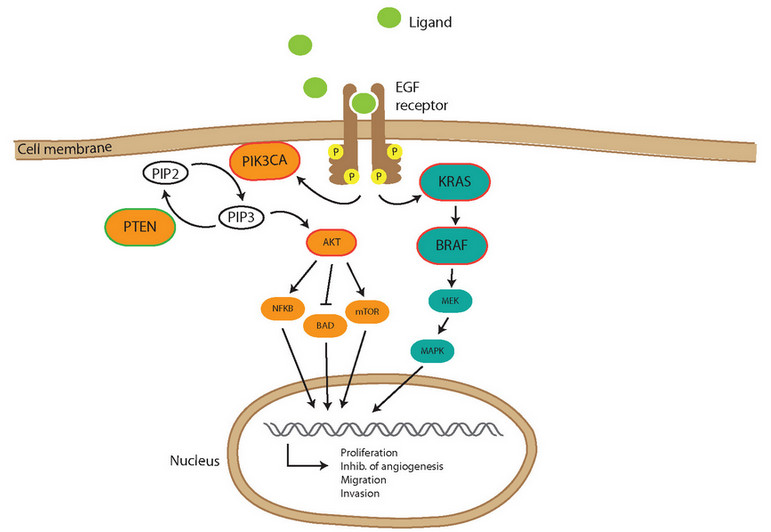
\includegraphics[scale=2.5,angle=0]{egfr_signaling.png}
        \caption{Schematic representation of the EGFR signaling cascade}}
      \end{center}
    \end{figure}

    \subsubsection{Biological Role of EGFR in Solid Tumors}

      The EGFR pathway is long known to be dysregulated in most solid tumors and
      thereby presents a rational target for cancer therapy. In normal cells,
      the tighly regulated EGFR signaling pathway drives cell-cycle progression,
      affects differentiation and migration and acts as a survival signal. EGFR
      levels have been shown to be higher in tumor samples than in surrounding
      tissues. Also, more of EGFR's ligands EGF and TGF$\alpha$ are found in
      these tumors. EGFR overexpression may result from epigenetic alterations
      or gene amplification. EGFR overexpression has been associated with poor
      prognosis if treated with classical chemotherapy, as this leads to a more
      aggressive progression.

      \paragraph{EGFR signaling as a survival signal:} Cells communicate with
      their environment. Without extracellular signals, a cell undergoes
      apoptosis. Signaling pathways induced by cell--matrix interactions,
      cell-cell interactions, and soluble survival factors act on a variety of
      genes and proteins. Loss of matrix attachment leads to cell growth arrest
      and cell death in normal epithelial cells, a process called anoikis. The
      cell--matrix interaction acts as a safeguard against inappropriate
      proliferation and migration.

      Activation of the EGFR signaling pathway protects normal epithelial
      cells against anoikis in the suspended state. EGFR blockade sensitizes
      normal epithelial cells to apoptosis, but the effect is much more
      pronounced in the suspended state than in the attached state. The
      redundancy of cell survival signals makes normal epithelial cells
      relatively resistant to EGFR-blockade in their normal microenvironment.

      Tumor cells are often in transit or at sites with inadequate matrix
      composition. They are often provided with inadequate or missing cell--cell
      and cell--matrix interactions. They are thereby more dependent on survival
      signals propagated by soluble mediators, such as EGF or TGF$\alpha$.
      Consequently, tumor cells are relatively sensitive against blockade of
      EGFR. This is counterbalanced by an upregulation of cell surface receptors
      that activate anti--apoptotic pathways. MAPK activation in the
      EGFR--activated RAS--RAF--MEK--ERK pathway is required for high expression
      of Bcl--XL, an anti-apoptotic protein of the Bcl--2 family. Bcl--2
      proteins regulate liberation of cytochrome c from the mitochondria, which
      is essential in the apoptotic caspase pathway. Additionally, EGFR
      signaling leads to post-transcriptional phosphorylation on the
      pro-apoptotic Bad protein, which is thereby functionally inactivated.

    \subsubsection{EGFR-targeted drugs}

      The observations that EGFR is recursively upregulated in many cancers and
      that EGFR is such an important mediator of cell-cycle progression,  cell
      growth, and cell survival, has lead to the development of agents that
      block this pathway. Pharmacologically, these agents can be classed by
      their mode of action: EGFR-targeted monoclonal antibodies and
      EGFR-specific tyrosine kinase inhibitors (TKIs). Several proteins acting
      downstream of EGFR are often found to be mutated. This lead to the
      development of other targeted drugs, such as BRAF-- or MEK--inhibitors.
      As many tumors are 'EGFR--addicted' and normal cells usually are provided
      with a redundancy of survival signals, these agents have less
      side--effects than classical cytotoxic chemotherapeutic agents.

       Anti--EGFR monoclonal antibodies bind to the extracellular domain of
      EGFR in its inactive state and thereby compete for EGF or TGF$\alpha$
      binding. They inhibit ligand-induced EGFR tyrosine kinase activation. The
      most popular anti--EGFR monoclonal antibody is cetuximab, whic binds to
      EGFR with a higher affinity than the natural ligands EGF or TGF$\alpha$.
      Binding of the antibody induces internalization of EGFR, following by its
      degradation. Cetuximab also binds to EGFRvIII, a constantly active
      version of EGFR. Cetuximab blocks cell--cycle  progression at the G0/G1
      boundary, inhibits cell proliferation and induces cancer cell death.

      EGFR-specific tyrosine kinase inhibitors comprise three classes, which
      include first generation reversible  EGFR-inhibitors (gefitinib,
      erlotinib), second generation irreversible inhibitors (afatinib,
      dacomitinib, neratinib) and third generation mutant-selective inhibitors
      (brigatinib, osimertinib, rociletinib). Third generation agents have a
      better sensitivity against mutated than wild-type EGFR and have been
      designed to further decrease treatment-associated side effects. TKIs are
      low molecular weight molecules that are mainly derived from quinazoline.
      These compounds bind to EGFR and block ligand-induced receptor
      phosphorylation by occluding the ATP--binding site. This results in
      inhibition of cell proliferation, cell--cycle arrest at the G0/G1 boundary
      and apoptosis.

    \subsubsection{Predictive markers}

      The mutational status of EGFR and downstream proteins is predictive of the
      potential success of EGFR-targeted therapy. Demonstration of the
      predictive value of these markers is not trivial and has to be proved in
      clinical trials. In many cases the predictive value of a marker, even
      though theoretically reasonable, has not yet been established. Currently,
      EGFR, KRAS, NRAS and BRAF are  used as predictive markers for
      EGFR--targeted therapy in solid tumors.

      \paragraph{EGFR} is a strong predictive biomarker for the success of the
      administration of EGFR-specific TKIs. EGFR activating mutations are
      observed in 10--35\% of NSCLC. 90\% of EGFR mutations are exon 19
      deletions (48\%) and exon 21 L585R (c.2573T$>$G) (43\%) point mutations.
      In melanoma and CRC, EGFR mutations are seldom. These mutations confer
      increased sensitivity to EGFR--specific tyrosine kinase inhibitors.
      Patients with EGFR--mutated tumors have a longer progression--free
      survival if treated with TKIs than those treated with traditional
      chemotherapy. Also, patients with EGFR--mutated tumors display a better
      prognosis if treated with EGFR TKIs compared to patients with wild--type
      EGFR cancers.

      \paragraph{KRAS} mutations are found in 36--40\% of CRCs, 15--25\% of
      NSCLC, and in 2\% of melanomas. Critical mutations in the KRAS gene
      include point mutations in codons 12, 13 and 61. Amongst these, the G12C
      variant is the most common. These mutations lock KRAS in its GTP-bound
      state, resulting in a constantly active protein, leading to a constantly
      active signal transduction. Blocking EGFR in that case is useless, as KRAS
      acts downstream of EGFR. KRAS activating mutations have been shown to
      confer reduced sensitivity to EGFR-targeted monoclonal antibodies in CRC
      and EGFR--TKIs in NSCLC.

      \paragraph{NRAS} is an isoform of KRAS. Activating mutations in NRAS
      codons 12 and 61 are found in 1--6\% of CRCs, 13--25\% of melanomas and
      1\% of NSCLCs. NRAS mutations have been associated with reduced
      sensitivity to EGFR monoclonal antibodies in CRC. The predictive value of
      the influence of NRAS mutations in NSCLC and melanoma has not yet been
      demonstrated in large clinical trials at this time.

      \paragraph{BRAF} mutations are very common in melanoma (37--50\%). 8--15\%
      of CRCs and 1--4\% of NSCLCs are BRAF--mutant positive. Amongst
      BRAF-mutated melanomas, the V600E variant is found in 80--90\% cases.
      V600E affects the activation segment of the BRAF kinase domain and results
      in an increased kinase activity. BRAF mutations usually confer a
      resistance to EGFR-targeted therapy in KRAS wild--type tumors. BRAF V600E
      mutations have been associated with increased sensitivity to BRAF
      inhibitors in melanoma and NSCLS and MEK inhibitors in melanoma.

  \subsection{Tumor DNA Sequencing}

     The completion of the Human Genome Project in 2001 resulted in a massive
    boost in molecular medicine. New high-throughput techniques, in combination
    with advanced computational performance and storage capacities, lead to an
    explosion of biological data. Amongst the many mutation detection
    techniques, Next--Generation Sequencing (NGS) constitutes the most powerful
    method and allows deep insights into the underlying causes of diseases.
    Even though advances in sequencing technology and computational power and
    tools have decreased the time and cost of a sequencing experiment, NGS is
    still mainly used in research, with only a few laboratories using this
    technique in diagnostics. NGS has profoundly impacted the field of
    oncology. A wide variety of NGS applications have been applied to study the
    genetics and epigenetics of cancer. ChIP--Seq and FAIRE--Seq allow
    determination of DNA--protein interactions and identification of DNA
    regulatory elements, respectively. The cancer transcriptome can be studied
    with RNA--Seq experiments. NGS has massively accelerated discovery of
    genetic and epigenetic alterations in tumors.

    The development of targeted NGS approaches have made it possible to
    implement NGS in clinical diagnostics laboratories. NGS allows deeper
    insights into the genetic sequences of oncogenes and tumor suppressor
    genes than array--based and single--gene approaches, which are currently
    used in most laboratories. Multiple genes can be studied in a single
    experiment, while classical methods are much more restricted in that
    regard. Targeted NGS experiments differ from whole--genome or whole--exome
    sequencing, as only a selection of regions of interest (ROIs) is captured
    and sequenced. This approach increases the efficiency of the experiment
    and the number of samples per run. Additionally, coverage, e.g. the number
    of sequencing reads that align to a specific base of the reference genome,
    is drastically increased in targeted NGS. This offers the sensitivity to
    detect low--frequency mutations in the tumor sample. Targeted NGS methods
    can be applied to study insertions, deletions and point mutations in genes
    of interest. NGS can thereby guide personalized cancer therapy by
    identifying the mutational status of genetic markers, which are predictive
    of the potential success of targeted cancer treatment.

    \subsubsection{Practical implications in the laboratory}

      Several studies have demonstrated the power of targeted NGS in the
      identification of the mutational status of EGFR, KRAS and BRAF. Comparison
      of NGS and real time PCR--based approaches showed high concordance of
      results. NGS was able to detect mutations that were not detectable by
      qPCR. Still, the implementation of new techniques into the workflow of molecular
      diagnostics laboratories requires a careful assessment of the sensitivity
      and sensibility of the method. The quality of tumor sequencing
      experiments is affected by several factors. These include the content of
      tumor cells in the sample, the quality of the tissue material, the choice
      of the sequencing library preparation kit and the bioinformatic pipeline.

      The tumor biopsy usually consists of an admixture of normal and cancer
      cells. The sensitivity of tumor variant detection is linked to the tumor
      cell content of the specimen. In addition, cancers are highly
      heterogeneous: a small subpopulation might present mutations, which
      provide resistance to the treatment. Detecting these low-frequency
      mutations and clearly delineating them from possible sample processing or
      sequencing induced artifacts presents an important challenge.

      Tumor biopsies usually yield a limited amount of tissue, therefore it is
      important to optimize sample usage by multiplexing analysis. In
      Luxembourg, all relevant tumor biopsies are sent to the
      Laboratoire National de Santé (LNS) to the Service of Pathologic Anatomy.
      Here, the biopsy is fixed in formalin and embedded in paraffin (FFPE).
      FFPE preserves the tissue morphology and thereby allows histological
      analysis. In addition, it allows specimen storage for decades. Sample
      quality, however, is influenced by this fixation method and the fixation
      time. DNA extraction from FFPE samples is difficult and yields low amounts
      of DNA; formaldehyde leads to cross-linking of nucleic acids and proteins;
      FFPE introduces fixation artifacts into DNA sequences, for instance C>T
      transitions. These circumstances complicate sample processing as well as
      NGS data interpretation. Though, FFPE samples have been shown to be still
      suitable for downstream PCR--based analyses.

      Several NGS bench-top devices have become available in the last decade.
      These instrumentations differ in their underlying chemistry that
      influences the instrument’s performance, accuracy, output and time per
      run. Common sequencing principles include pyrosequencing (454), sequencing
      by ligation (SOLiD), ion semiconductor sequencing (Ion Torrent) and
      sequencing by synthesis (Illumina).

      Sequencing library preparation also affects the final NGS result. Several
      technologies for target enrichment exist and are available for different
      sequencing instruments. Two steps are essential for all these enrichment
      methods: target sequences have to be enriched and samples have to be
      multiplexed, which requires the incorporation of a unique index
      combination for each sample. Target enrichment methods can be separated
      into three basic groups: targeted circularization, hybrid capture of
      target fragments and PCR-based enrichment methods. Multiplex PCR--based
      approaches produce short DNA fragments of target regions in a first PCR.
      In a second PCR, adapters and indices are added. Hybridization--based
      methods require a so-called shotgun library construction before target
      regions can be captured. During this process, genomic DNA is randomly
      sheared into small fragments and an adapter-- and index--linked library is
      produced. Biotinylated baits are added that bind to target sequences.
      Target regions can then be captured using streptadivin coated magnetic
      beads. Targeted circularization methods rely on a digestion of DNA by
      restriction enzymes. The produced DNA fragments are circularized and
      captured. Only circularized target are then amplified by PCR.

      The establishment and validation of a bioinformatic NGS data analysis
      pipeline still presents a challenge in diagnostics. After generation of
      FASTQ files of the sequencer, data generally undergo quality control,
      followed by trimming of low quality bases, alignment to the reference
      genome, variant calling and variant annotation. For each of these steps,
      several bioinformatic algorithms and tools exist. The computational
      pipeline of the molecular pathology laboratory has to incorporate the
      tools that allow the most sensitive and sensible analysis of data. For
      instance, quality trimming influences the mapping to the reference genome.
      The mapping, in turn, strongly affects the variant calling. In fact,
      variant calling is a critical step in NGS data analysis. Several variant
      calling tools exist, but vary in their false-positive and false-negative
      detection rates. These tools have to be carefully assessed, as
      false-positives or false-negatives should absolutely be avoided when it
      comes to the prescription of a targeted chemotherapeutic agent.

      To facilitate interpretation of NGS data, variants have to be annotated
      and their clinical actionability has to be identified. Several databases
      have emerged in this field and numerous
      tools allow to automatize variant annotation. Here again, the choice of
      the database and the variant annotator is important.

      Finally, the sample--to--results time is a very pragmatic, but important
      factor. The time from the biopsy to the potential start of an
      administration of a targeted chemotherapeutic drug should be reduced to a
      reasonable minimum. For instance, in case of late--stage cancer patients,
      it would be unacceptable if analysis would take several weeks. To reduce
      the sample--to--results time, the sample processing
      workflow should be as short as possible, while still yielding high quality
      sequencing libraries. The bioinformatic pipeline should not only
      incorporate the best tools, but should also be automatized to further
      reduce the time of analysis.

  \subsection{Aims of the Thesis}
